\chapter[2024 April]{April 2024}

\section{April Schedule}

\TabRef{tab:schedule_04} Shows the EPR 402 schedule for April 2024.
\begin{table}[H]
  \centering
  \caption{EPR 402 Schedule for April 2024}
  \label{tab:schedule_04}
    \begin{tabular}{ !{\vrule width 1.1pt}
                    c!{\vrule width 1pt}
                    c!{\vrule width 1pt}
                    c!{\vrule width 1pt}
                    p{8.6cm}!{\vrule width 1pt}}
    \noalign{\hrule height 1pt}
    \cellcolor[gray]{0.9} \textbf{Week} &
    \cellcolor[gray]{0.9} \textbf{Date} &
    \cellcolor[gray]{0.9} \textbf{Part} &
    \cellcolor[gray]{0.9} \textbf{Required reading / Assignment due date }
    \\ \noalign{\hrule height 1pt}
    4     &  2 Apr --   5 Apr & 1 & Research different processing platforms.
    \\ \hline
    5     &  8 Apr --   12 Apr & 1 & Test Week - Project proposal draft 1st Revision
    \\ \hline
    6     &  15 Apr --   19 Apr & 1 & Project Proposal draft 2nd revision
    \\ \hline
    7     &  22 Apr --   26 Apr & 1 & Project Proposal draft final revision
    \\ \hline
    8     &  29 Apr --   30 Apr & 1 & Project proposal due
    \\ \noalign{\hrule height 1pt}
    \end{tabular}
\end{table}

\pendsign

\subsection{This is a sample heading, typically activity related}

Some normal text....

\subsection{Approach: Lab book}

Some normal text....

\begin{slantnote}
  Keeping a lab notebook is generally considered best practice, both for
  engineering work and also research projects such as this. A paper based
  approach is however less than ideal as the resultant work cannot be
  easily searched. For work of this nature it has further disadvantages
  with respect to figures, plots and code fragments being harder to manage
  given that all three are to be generated automatically.

  A ``year+month'' based hierarchy was decided on in order to balance the
  complexity of organisation and the level of nesting. For the cases where
  additional files must be included. As a result of the nesting however the
  \LaTeX\ \texttt{$\backslash$input} command must be used to handle the
  inclusion.
\end{slantnote}

Some normal text....

\pendsign

\section[2024/04/04]{Thursday, 3 April 2024}

\subsection{Research Ideas}

\begin{compactitem}
\item Idea 1... testing acronym \ac{EM}
\item Idea 2... testing index \bidx{SLAM}
\item Idea 3... testing href and reference
\href{http://en.wikipedia.org/wiki/David_Marr_(neuroscientist)}{David Marr}
\index{Marr, David}~\cite{marr_aa_2010}
\end{compactitem}

\todoredefined{Should do a search to identify any relevant ... }

\EquRef{eqn:example} shows an example of a numbered equation.
\begin{equation}
  \Delta w_{i,j} = \alpha a_i \Delta[j]  \label{eqn:example}
\end{equation}
A subsection a subsection a subsection a subsection a subsection a
subsection a subsection a subsection a subsection a subsection a
subsection a subsection a subsection a subsection a subsection.
\nocite{dellaert_spieits_1997}

\FigRef{fig:example} shows an example of a figure.
\begin{figure}[!ht]
  \centering
  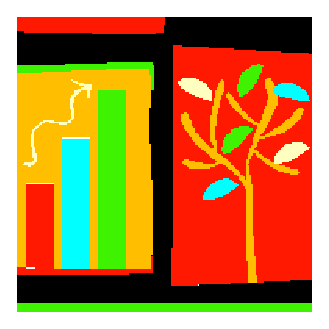
\includegraphics[width=0.4\linewidth]{figures/figure1}
  \caption{This is a figure caption}
  \label{fig:example}
\end{figure}

Third theme of literature study third theme of literature study third
theme of literature study third theme of literature study. See
\SecRef{sec:somewhere} for more information.
